%-------------------------------------------------------------------------
% Section: our main work
%-------------------------------------------------------------------------

\chapter{Proposed solution }
\label{cha:proposed solution }


\begin{figure}[!htb]
  \centering
  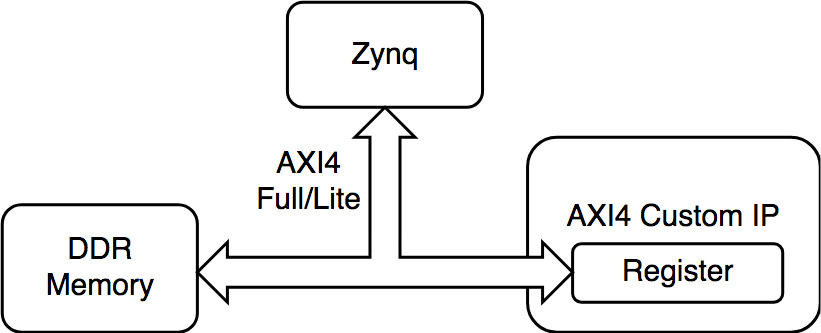
\includegraphics[scale=0.5]{images/AXI4customIP.jpg}
  \caption[Custom IP with AXI4-Lite/Full Register.]{Custom IP with AXI4-Lite/Full Register.}
  \label{fig:Custom IP with AXI4-Lite/Full Register.}
\end{figure}

%-------------------------------------------------------------------------
% Section: 
%-------------------------------------------------------------------------

\section{Linux UIO driver for AXI DMA}
\label{sec:Linux UIO driver for AXI DMA}

\subsection{Scatter Gather}
\label{subsec:Scatter Gather}
In tranditional DMA transaction, it can only accept a contiguous (nonsegmented) block of
physical memory, so, if we want to use DMA in userspace, and we can not get a contiguous 
memory space(like CMA), then we need to use DMA Scatter/Gather mode. This mode allows non-
contiguous (nonsegmented) block of physical memory and this mode need to be turn on in Vivado 
design first. In this mode, DMA controller automatically give the start address of the 
segmented of memory after the previous transaction of segmented memory is completed. To 
apply this mode, we need to construct a special data structure, Scatterlist, which collects 
start address and lengths of segmented block of user buffer memory. DMA engine will do the
transaction according to this list. 


\subsection{Cache Coherency}
\label{subsec:Cache Coherency}
While using DMA to do the data transfering, it may lead cache coherency problems. Figure~\ref{fig:Cache Coherency Problems.}
shows the cache coherency problem, both read and write may lead this problem, so if we want to 
transfer correct data, we must solve this problem.

My first trial is try to solve this problem in user application, that is, announce ``volatile'' 
buffer to prevents an optimizing compiler from optimizing away subsequent reads or writes and 
thus incorrectly reusing a stale value or omitting writes. 
\begin{figure}[!htb]
  \centering
  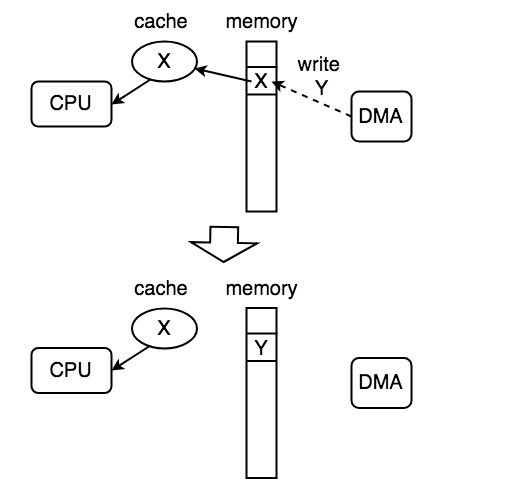
\includegraphics[scale=0.5]{images/cache_coherency.jpg}
  \caption[Cache Coherency Problems.]{Cache Coherency Problems.}
  \label{fig:Cache Coherency Problems.}
\end{figure}
%-------------------------------------------------------------------------
% Section: 圖表
%-------------------------------------------------------------------------

\section{Implementation}
\label{sec:Implementation}




